%!TEX root = ../professor.tex
\chapter{Para o professor}\label{chap3}

Esta lição retoma a reta numérica como uma representação organizada para os números. Objetiva-se a inclusão das frações nessa representação. Assim, espera-se do aluno maior abstração: agora a fração não é mais apenas ``fração da unidade'' mas também quantidade, um número. Espera-se ainda que os alunos reconheçam a evidência da ordem na reta numérica .

A comparação de frações, já discutida em atividades nas lições anteriores, pode agora ser também observada a partir da reta numérica, embora seja sistematizada apenas na \hyperref[chap4]{Lição 4}. Pretende-se aqui abordar a comparação de frações de mesmo denominador, de mesmo numerador e a partir de um referencial. 

Neste livro, o conceito de fração foi construído a partir da equipartição e fortemente amparado por modelos concretos ou de área. Assim, até aqui, faz sentido dizer ``dois terços da unidade'', sendo a unidade explicitamente identificada: por exemplo, dois terços de pizza, dois terços de uma região ou dois terços de um objeto. Esta lição propõe um avanço no sentido da abstração. Espera-se que $\frac{2}{3}$ seja reconhecido como um número, pressupondo uma unidade abstrata. Poder-se-á falar em ``o número dois terços'' ou que ``dois terços é maior que meio'' sem que seja especificada a unidade (pizza, quadrado, círculo etc.). Observa-se que esse caminho é análogo ao já trilhado para os números naturais, que, inicialmente associados à contagem de objetos concretos ($2$ laranjas, por exemplo), quando munidos da abstração, passam a ser comparados e somados sem que se identifique explicitamente a unidade: Sabemos que $2$ é menor do que $3$ e $2 + 3 = 5$ seja a unidade uma formiga, uma cadeira ou um disco voador. Espera-se que os alunos entendam, façam uso de, comparem e operem com frações como números. A representação na reta numérica é um aporte importante para isso.

O caminho para a abstração aqui proposto baseia-se na associação da unidade a um segmento denominado segmento unitário, mais especificamente ao segmento de extremidades zero e um. Deste modo, na reta numérica, o segmento unitário é um modelo abstrato contínuo para qualquer unidade considerada.
\vspace{.2cm}

\begin{minipage}{\textwidth}
\begin{multicols}{2}
% \noindent \begin{tabular}{e{.17\linewidth}e{.17\linewidth}e{.17\linewidth}e{.3\linewidth}}
% 
\includegraphics[width=40pt,keepaspectratio]{licao03/pizza.png} & \begin{tikzpicture}[x=25mm,y=25mm]
% \def\scale{.37}% to rescale the polygons only.

% %hexagon on the right
% \foreach \x in {30,90,...,330}{
% \draw[shift={(1,0.6)}, fill=attention,attention, scale=\scale] (\x:0.7) -- (\x + 60: 0.7) --(0,0) --cycle;
% \draw[shift={(1,0.6)}, fill=attention, scale=\scale] (\x:0.7) -- (\x + 60: 0.7);}
% \end{tikzpicture} &
% 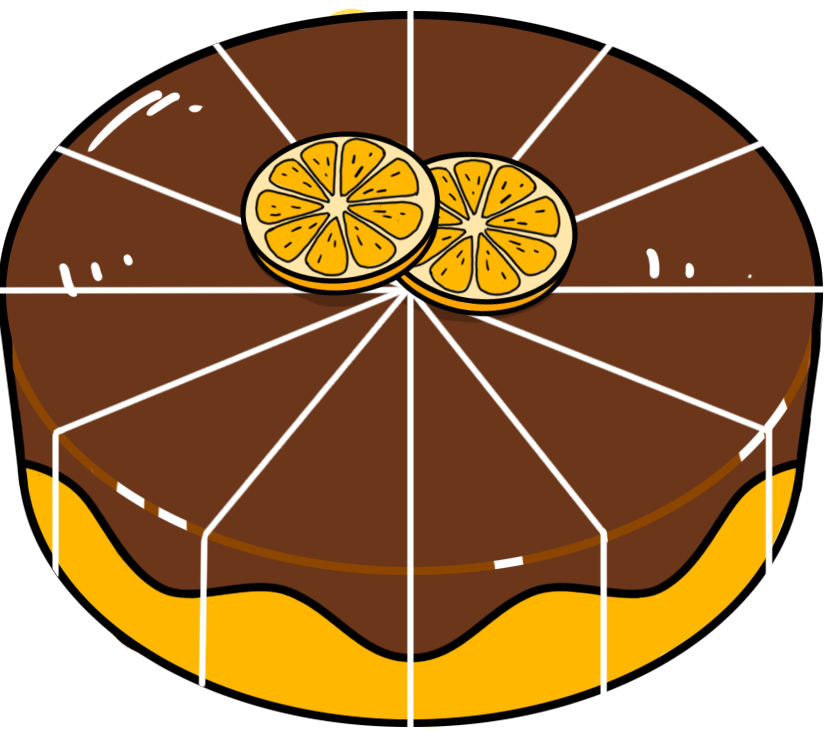
\includegraphics[width=40pt,keepaspectratio]{licao03/ativ4_fig_e.png} &
% \resizebox{\linewidth}{!}
% {
% \begin{tikzpicture}[x=1mm,y=1mm, scale=.4]
 
%   \draw[fill=attention] (0,0) rectangle (75,10);
%   \foreach \x in {15,30,45,60,75}{ \draw (\x,0) -- (\x,10);}

% \end{tikzpicture}
% }
%           \end{tabular}
\null\vfill
\begin{figure}[H]
\centering

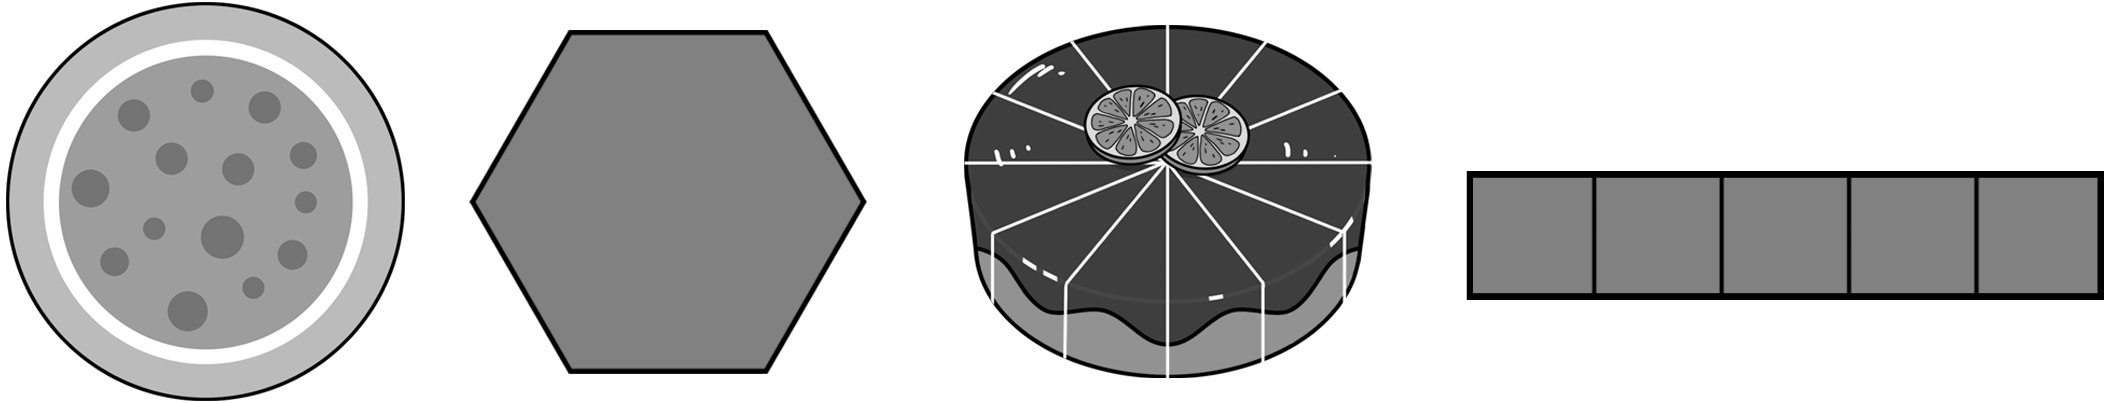
\includegraphics[width=.8\linewidth]{licao03/introducao-professor}
\end{figure}
\vfill\null

\columnbreak

\null\vfill
\begin{center}

 \begin{tikzpicture}[x=15mm,y=15mm]
\node[above] at (.5,3pt) {unidade};
\draw[->] (-0.5,0) -- (3.5,0) ; %edit here for the axis
\foreach \x in {0,1}{ \node[below] at (\x,-3pt) {\x};}
\draw[very thick, attention] (0,0) -- (1,0);
\foreach \x in {0,1}{ \fill[attention] (\x,0) circle (3pt);}
\end{tikzpicture}

\end{center}

\vfill\null
\end{multicols}
\end{minipage}

Assim como feito com as unidades representadas pictórica ou abstratamente até aqui, o segmento unitário será repartido em partes iguais, que determinarão as frações unitárias e essas partes serão  reunidas para determinar novas frações da unidade. O registro das frações na reta numérica é feito de forma análoga ao dos números naturais. Por exemplo, para se marcar $4$ na reta numérica são justapostas $4$ unidades a partir do zero e no final marca-se o ponto correspondente ao número $4$. Para se marcar o $\frac{4}{3}$ na reta numérica, são justapostos $4$ terços da unidade a partir do zero e no final marca-se o número~$\frac{4}{3}$.

\begin{multicols}{2}
\begin{center}
%7 unidades
\begin{tikzpicture}[x=15mm,y=18mm]

\draw[->] (-0.25,0) -- (4.75,0) ; %reta 
\draw[very thick, attention] (0,0) -- (4,0);
\node[above] at (2 , 3pt) {4 unidades};

\foreach \x in {1,2,3,4}{ \draw (\x,3pt) -- (\x,-3pt) node[below] {\x};}

\foreach \x in {0,4}
{
  \fill[attention] (\x,0) circle (3pt);
  \node[below] at (\x,-3pt) {\x};
}
\end{tikzpicture}

  %1/3 da unidade
  \begin{tikzpicture}[x=15mm,y=18mm]
\draw[->] (-0.25,0) -- (2,0) ; %reta anterior
\draw[very thick, attention] (0,0) -- (1/3,0);
\node[above] at (1/6,3pt) {$\frac{1}{3}$ da unidade};
\foreach \x in {0,1}{ \draw (\x,3pt) -- (\x,-3pt) node[below] {\x};}

\draw (2/3,3pt) -- (2/3,-3pt);
\node[below] at (1/3,-3pt) {$\dfrac{1}{3}$};
\foreach \x in {0,1/3}{ \fill[attention] (\x,0) circle (3pt);}
%\fill[common] (1/3,0) circle (3pt);
\end{tikzpicture}\quad\quad
%4/3 da unidade
\begin{tikzpicture}[x=15mm,y=18mm]
\draw[->] (-0.25,0) -- (2,0) ; %reta anterior
\draw[very thick, attention] (0,0) -- (4/3,0);
\foreach \x in {0,1}{ \draw (\x,3pt) -- (\x,-3pt) node[below] {\x};}

\draw (1/3,-3pt) -- (1/3,3pt);
\draw (2/3,3pt) -- (2/3,-3pt);
\node[below] at (1/3,-3pt) {$\dfrac{1}{3}$};
\node[below] at (2/3,-3pt) {$\dfrac{2}{3}$};
\node[below] at (4/3,-3pt) {$\dfrac{4}{3}$};

\node[above] at (2/3,3pt) {$\frac{4}{3}$ da unidade};

\foreach \x in {0,4/3}{ \fill[attention] (\x,0) circle (3pt);}
\end{tikzpicture}
\end{center}
\end{multicols}




A reta numérica é um modelo visual poderoso e universal que suporta a ampliação dos diferentes conjuntos de números (dos naturais aos reais, passando pelas frações, números inteiros e pelos números racionais) ao longo dos anos de escolaridade. Em particular a ordem fica evidente na reta numérica a partir da organização dos números. Obedece-se a ordem crescente no sentido que vai do zero para o um. Se considerados dois números e a organização obedecendo o sentido crescente, o menor será aquele que vier antes. Por exemplo, nas imagens a seguir $a$ é menor do que $b$ e $c$ é maior do que $d$.

\begin{center}
 \begin{tikzpicture}[x=18mm,y=18mm,scale=.6]
\draw[->] (-0.5,0) -- (3.5,0) ; %edit here for the axis
\foreach \x in {0,1}{\node[below] at (\x,-3pt) {$\x$};}
%\draw[very thick, attention] (0,0) -- (1,0);
\foreach \x in {0,1}
{
\draw (\x,3pt) -- (\x,-3pt);
}
\foreach \x/\c/\n in {1.2/attention/a,2/attention/b}
{
  \fill [\c] (\x,0) circle (3pt);
  \node [below] at (\x,-3pt) {$\n$};
}

\end{tikzpicture}
\hspace{3em}
 \begin{tikzpicture}[x=18mm,y=18mm, rotate=-15, scale=.6]
\draw[->] (-0.5,0) -- (3.5,0) ; %edit here for the axis
\foreach \x in {0,1}{\node[below] at (\x,-3pt) {$\x$};}
%\draw[very thick, attention] (0,0) -- (1,0);
\foreach \x in {0,1}
{
\draw (\x,3pt) -- (\x,-3pt);
}
\foreach \x/\c/\n in {0.8/attention/d,1.6/attention/c}
{
  \fill [\c] (\x,0) circle (3pt);
  \node [below] at (\x,-3pt) {$\n$};
}

\end{tikzpicture}
\end{center}

Nesta lição, a comparação de frações é estudada particularmente em três casos:
\begin{itemize}
\item \textit{Frações de mesmo denominador:} por exemplo, a fração $\frac{3}{4}$ é menor do que a fração $\frac{7}{4}$ uma vez que a primeira fração corresponde à justaposição de $3$ segmentos iguais a $\frac{1}{4}$ da unidade e a segunda à justaposição de $7$ desses segmentos. Dessa forma, $\frac{3}{4}$ é menor do que $\frac{7}{4}$ e pelo mesmo motivo, na reta numérica, o $\frac{7}{4}$ está mais à direita do zero do que $\frac{3}{4}$.
\item \textit{Frações com mesmo numerador:}  por exemplo, a fração $\frac{5}{7}$ é menor do que $\frac{5}{3}$ porque nos dois casos considera-se a justaposição de $5$ segmentos, no entanto, no primeiro caso, são $5$ segmentos de $\frac{1}{7}$ da unidade e, no segundo, de $\frac{1}{3}$ da unidade. Como $\frac{1}{7}$ da unidade é menor do que $\frac{1}{3}$ da unidade, tem-se que $\frac{5}{7}$ é menor do que $\frac{5}{3}$.
\item \textit{A partir de um referencial:} por exemplo, a fração $\frac{7}{8}$ é menor do que a fração $\frac{8}{9}$ porque, apesar de ambos estarem associados a pontos à esquerda do $1$, o ponto correspondente à fração $\frac{7}{8}$ está mais distante do $1$ (a $\frac{1}{8}$ de distância) do que o correspondente à fração $\frac{8}{9}$ (que está a $\frac{1}{9}$ de distância do $1$).
\end{itemize}


\section{Objetivos específicos da Lição 3}
\paragraph{O aluno deve ser capaz de:}


  \begin{itemize}
   \item Representar e identificar a representação de uma fração na reta numérica (Atividades \ref{chap3-ativ1} a \ref{chap3-ativ13}, \ref{chap3-ativ15}, \ref{chap3-ativ17} e \ref{chap3-ativ18}). 
   \item Reconhecer a organização das frações na reta numérica segundo a ordem (Atividades \ref{chap3-ativ8}, \ref{chap3-ativ9}, \ref{chap3-ativ17} e \ref{chap3-ativ18}). 
   \item Comparar frações com mesmo numerador ou mesmo denominador (Atividades \ref{chap3-ativ7}, \ref{chap3-ativ8}, \ref{chap3-ativ13} a \ref{chap3-ativ16}).
   \item Comparar frações a partir de um referencial adequado, amparado pela representação na reta numérica (Atividades \ref{chap3-ativ12}, \ref{chap3-ativ16} e \ref{chap3-ativ17}).
\item Compreender frações como números (Atividades \ref{chap3-ativ5}, \ref{chap3-ativ10} a \ref{chap3-ativ16} e \ref{chap3-ativ18}). 
  \end{itemize}

\textbf{Recomendação:}  Nas atividades desta lição, salvo orientação específica, recomenda-se que os alunos trabalhem individualmente ou em duplas e que as diferentes soluções sejam discutidas com toda a turma. Estimule seus alunos a explicarem suas respostas.


\begin{atividade}\label{chap3-ativ1}
\objetivos
\begin{itemize} %s
    \item Reconhecer a representação de frações na reta numérica a partir da graduação em uma escala linear.
    \item Associar,  na reta numérica, o segmento unitário à unidade.
    \item Reconhecer a representação de frações do segmento unitário na reta numérica.
\end{itemize} %s

\discussoes
\begin{itemize} %s
\item Espera-se que os alunos (i) associem o 0 (zero) à caixa d'água vazia e o 1 (um) à caixa cheia; (ii) Descartem as faixas (c) e (d) porque não respeitam a equipartição e que (iii) reconheçam que as faixas a), b) e e) são marcações possíveis. Discuta com os alunos as vantagens e as desvantagens dessas marcações. A faixa a) traz a marcação da fração $\frac{1}{2}$ associada ao segmento e não ao ponto, o que dificulta a indicação de alturas intermediárias, como $\frac{1}{4}$, por exemplo. A faixa (e) tem poucas marcações, limitando a medição.
\item A atividade aborda a medição de volume a partir de uma escala linear. Os alunos precisam reconhecer que a quantidade de água no recipiente está associada à altura do líquido no recipiente. Para garantir que os alunos compreendam o processo, considere mostrar a eles um recipiente transparente na forma de um paralelepípedo ou de um cilindro e fazer perguntas como ``até onde eu preciso encher para alcançar metade da capacidade? E um quinto?''.
\item Observe que o formato da caixa, um paralelepípedo, possibilita uma escala linear para a medida do volume (o mesmo valeria para um cilindro, por exemplo). No entanto, para outros formatos de caixa, esse mesmo tipo de escala não seria adequado. É o caso, por exemplo, de um cone. Uma tal discussão foge aos objetivos do estudo de frações.
\end{itemize} %s

\solucao
  A faixa graduada b) é a mais indicada para registrar as quantidades de todos os momentos porque possui marcações com mesmo espaçamento, na ordem adequada e com informações claras para os quatro momentos. A graduação e), ainda que correta, só permite a leitura da quantidade de água nos momentos 2 e 4. Já a graduação a) tem a marcação $\frac{1}{2}$ associada ao segmento e não à um ponto, o que dificulta leituras intermediárias. A graduação c) não respeita a equipartição porque possui a marca $\frac{1}{2}$ em um ponto acima da metade da altura da caixa. Já na faixa graduada d) as marcações não respeitam a ordem, a marca $\frac{1}{2}$ é alcançada antes da marca $\frac{1}{3}$. 

\end{atividade}

\begin{atividade}\label{chap3-ativ2}
\objetivos
\begin{itemize} %s
    \item Recordar a reta numérica, associando quantidades inteiras aos números naturais. Em particular, objetiva-se que a unidade seja associada ao número 1.
    \item Representar frações na reta numérica.
\end{itemize} %s

\discussoes
\begin{itemize} %s
    \item        Recomenda-se que o professor inicie a atividade relembrando com os alunos como é construída a reta numérica e como se posicionam os números naturais nela, enfatizando que uma vez escolhidos os pontos que vão representar 0 e 1 (tipicamente, com o ponto que representa 1 à direita do ponto que representa 0), todos os demais números naturais têm suas posições estabelecidas por meio de justaposições de segmentos iguais ao segmento cujas extremidades são os pontos que representam 0 e 1.
    \item       Espera-se que os alunos, a partir de tal revisão, não tenham dificuldade para resolver o item a). A novidade está no item b), no qual os alunos são solicitados a representar frações na reta numérica. Nesse item, o objetivo é que os alunos concluam que, na reta numérica, assim como o ponto correspondente ao 2 fica determinado pela justaposição de dois segmentos unitários e que o ponto correspondente ao 3 fica determinado pela justaposição de três segmentos unitários, o ponto correspondente a $\frac{1}{2}$ é o ponto médio do segmento unitário. De forma análoga, considerando equipartições do segmento unitário e a justaposição dessas partes, são determinados, por exemplo, os pontos correpondentes às fraçoes $\frac{1}{4}$ e $\frac{3}{4}$.
\end{itemize} %s

\end{multicols}

\clearpage
\solucao

\begin{multicols}{2}

\begin{enumerate}
\item \adjustbox{valign=t}
{
\begin{tikzpicture}[x=10mm,y=10mm]
\draw[->] (-1,0) -- (6,0) ; %edit here for the axis
\foreach \x in  {0,1,...,5} % edit here for the vertical lines
\draw[shift={(\x,0)},color=black] (0,3pt) -- (0pt,-3pt)
node[below] {$\x$};
\foreach \x in {1,2,4}
\fill[common] (\x,0) circle (3pt);
\node at (1,9pt) {(A)};
\node at (2,9pt) {(B)};
\node at (4,9pt) {(C)};
\end{tikzpicture}
}

\item \adjustbox{valign=t}
{
\begin{tikzpicture}[x=25mm,y=25mm]
\draw[->] (-1/4,0) -- (2.5,0) ; %edit here for the axis
\foreach \x in  {0,0.25,...,2} % edit here for the vertical lines
\draw[shift={(\x,0)},color=black] (0,3pt) -- (0pt,-3pt);
\foreach \x in  {0,1,2}
\draw[shift={(\x,0)},color=black] (0,3pt) -- (0pt,-3pt) node[below] {$\x$};

\foreach \x in {1,3}
\fill[common] (\x/2,0) circle (3pt) node[below, black] {$\frac{\x}{2}$};

\foreach \x in {1,3}
\fill[common] (\x/4,0) circle (3pt) node[below, black] {$\frac{\x}{4}$};

\node at (.5,9pt) {(D)};
\node at (.25,9pt) {(E)};
\node at (.75,9pt) {(F)};
\node at (1.5,9pt) {(G)};
\end{tikzpicture}
}
\end{enumerate}

\end{atividade}

\begin{atividade}\label{chap3-ativ3}
\objetivos
\begin{itemize} %s
    \item       Associar frações representadas em modelos contínuos, com unidades variadas, à representação dessas fracões na reta numérica.
\end{itemize} %s

\discussoes
\begin{itemize} %s
    \item       Aproveite as imagens e faça perguntas à turma que explorem conteúdos já tratados anteriormente, tais como: a) Que fração da pizza foi comida? b) Essa quantidade de chocolate é maior, menor ou igual a meia barra de chocolate? c) Se a maçã estivesse inteira, que ponto da reta representaria tal quantidade?
\end{itemize} %s

\solucao
\begin{enumerate}
\item \adjustbox{valign=t}
{
\begin{tikzpicture}[x=40mm,y=60mm]
\draw[->] (-1/4,0) -- (1+1/4,0) ; %edit here for the axis
\foreach \x in  {0,0.5,1}{ % edit here for the vertical lines
\draw[shift={(\x,0)},color=black] (0,3pt) -- (0pt,-3pt);}
\foreach \x in  {0,1}
\draw[shift={(\x,0)},color=black] (0,3pt) -- (0pt,-3pt) node[below] {$\x$};
\draw[shift={(.5,0)},color=black] (0,3pt) -- (0pt,-3pt) node[below] {$\frac{1}{2}$};

\fill[common] (.5,0) circle (3pt);

\end{tikzpicture}
}

\item \adjustbox{valign=t}
{
\begin{tikzpicture}[x=37.5mm,y=56.25mm]
\draw[->] (-0.3,0) -- (1.3,0) ; %edit here for the axis
\foreach \x in  {0,1} % edit here for the vertical lines
\draw[shift={(\x,0)},color=black] (0,3pt) -- (0pt,-3pt)
node[below] {$\x$};

\foreach \x in {3,5}{
\draw[shift={(\x/8,0)},color=black] (0,3pt) -- (0pt,-3pt)
node[below] {$\frac{\x}{8}$};}
\fill[common] (5/8,0) circle (3pt);

\end{tikzpicture}
}

\item \adjustbox{valign=t}
{
\begin{tikzpicture}[x=37.5mm,y=56.25mm]
\draw[->] (-0.3,0) -- (1.3,0) ; %edit here for the axis
\foreach \x in  {0,1} % edit here for the vertical lines
\draw[shift={(\x,0)},color=black] (0,3pt) -- (0pt,-3pt)
node[below] {$\x$};

\foreach \x in {3,5}{
\draw[shift={(\x/8,0)},color=black] (0,3pt) -- (0pt,-3pt)
node[below] {$\frac{\x}{8}$};}
\fill[common] (5/8,0) circle (3pt);

\end{tikzpicture}
}


\item \adjustbox{valign=t}
{
\begin{tikzpicture}[x=40mm,y=60mm]
\draw[->] (-1/4,0) -- (1+1/4,0) ; %edit here for the axis
\foreach \x in  {0,0.25,...,1}{ % edit here for the vertical lines
\draw[shift={(\x,0)},color=black] (0,3pt) -- (0pt,-3pt);}
\foreach \x in  {0,1}
\draw[shift={(\x,0)},color=black] (0,3pt) -- (0pt,-3pt) node[below] {$\x$};
\foreach \x in  {1,3}
\draw[shift={(\x/4,0)},color=black] (0,3pt) -- (0pt,-3pt) node[below] {$\frac{\x}{4}$};
\draw[shift={(.5,0)},color=black] (0,3pt) -- (0pt,-3pt) node[below] {$\frac{1}{2}$};

\fill[common] (.5,0) circle (3pt);

\end{tikzpicture}
}

\item \adjustbox{valign=t}
{
\begin{tikzpicture}[x=40mm,y=60mm]
\draw[->] (-1/4,0) -- (1+1/4,0) ; %edit here for the axis
\foreach \x in  {0,0.25,...,1}{ % edit here for the vertical lines
\draw[shift={(\x,0)},color=black] (0,3pt) -- (0pt,-3pt);}
\foreach \x in  {0,1}
\draw[shift={(\x,0)},color=black] (0,3pt) -- (0pt,-3pt) node[below] {$\x$};
\foreach \x in  {1,3}
\draw[shift={(\x/4,0)},color=black] (0,3pt) -- (0pt,-3pt) node[below] {$\frac{\x}{4}$};
\draw[shift={(.5,0)},color=black] (0,3pt) -- (0pt,-3pt) node[below] {$\frac{1}{2}$};

\fill[common] (.25,0) circle (3pt);

\end{tikzpicture}
}

\item \adjustbox{valign=t}
{
\begin{tikzpicture}[x=12.9mm,y=25.71mm]
\draw[->] (-.5,0) -- (3,0) ; %edit here for the axis
\foreach \x in  {0,0.5,...,2.5}{ % edit here for the vertical lines
\draw[shift={(\x,0)},color=black] (0,3pt) -- (0pt,-3pt);}
\foreach \x in  {0,1,2}
\draw[shift={(\x,0)},color=black] (0,3pt) -- (0pt,-3pt) node[below] {$\x$};
\foreach \x in  {1,3,5}
\draw[shift={(\x/2,0)},color=black] (0,3pt) -- (0pt,-3pt) node[below] {$\frac{\x}{2}$};

\fill[common] (1,0) circle (3pt);

\end{tikzpicture}
}

\item \adjustbox{valign=t}
{
\begin{tikzpicture}[x=12.9mm,y=25.71mm]
\draw[->] (-.5,0) -- (3,0) ; %edit here for the axis
\foreach \x in  {0,0.5,...,2.5}{ % edit here for the vertical lines
\draw[shift={(\x,0)},color=black] (0,3pt) -- (0pt,-3pt);}
\foreach \x in  {0,1,2}
\draw[shift={(\x,0)},color=black] (0,3pt) -- (0pt,-3pt) node[below] {$\x$};
\foreach \x in  {1,3,5}
\draw[shift={(\x/2,0)},color=black] (0,3pt) -- (0pt,-3pt) node[below] {$\frac{\x}{2}$};

\fill[common] (2.5,0) circle (3pt);

\end{tikzpicture}
}

\item \adjustbox{valign=t}
{
\begin{tikzpicture}[x=12.9mm,y=25.71mm]
\draw[->] (-.5,0) -- (3,0) ; %edit here for the axis
\foreach \x in  {0,0.5,...,2.5}{ % edit here for the vertical lines
\draw[shift={(\x,0)},color=black] (0,3pt) -- (0pt,-3pt);}
\foreach \x in  {0,1,2}
\draw[shift={(\x,0)},color=black] (0,3pt) -- (0pt,-3pt) node[below] {$\x$};
\foreach \x in  {1,3,5}
\draw[shift={(\x/2,0)},color=black] (0,3pt) -- (0pt,-3pt) node[below] {$\frac{\x}{2}$};

\fill[common] (0,0) circle (3pt);
\end{tikzpicture}
}
\end{enumerate}


\end{atividade}

\anotacoes


\begin{atividade}\label{chap3-ativ4}
\objetivos
\begin{itemize} %s
    \item Representar frações na reta numérica.
    \item Associar, na reta numérica e a partir de modelos contínuos, a unidade ao número 1.
\end{itemize} %s

\discussoes
\begin{itemize} %s
    \item       Esta atividade propõe, a partir de modelos contínuos, a associação de quantidades a pontos da reta numérica. Para isso, em cada item estão destacados na reta, além do 0 e do 1, frações e marcações apropriadas às subdivisões correspondentes. Por exemplo, para o quadrado que  está dividido em nonos, o segmento unitário traz uma marcação que destaca a subdivisão em nove partes iguais e destaca as frações $\frac{4}{9}$ e $\frac{5}{9}$.
    \item Para responder, o aluno pode simplesmente ligar com uma linha a representação em imagem ao ponto da reta correspondente à fracão identificada.
    \item Observe que o enunciado não determina a unidade. É provável que o aluno escolha as regiões totalmente coloridas em vermelho como unidade. A solução considera esse caso. No entanto, a região colorida em vermelho de qualquer uma das figuras pode ser considerada unidade. Essa escolha torna a solução mais complexa nos itens c) e f). Por exemplo, no item c), se a região em vermelho da Figura A for a unidade, a Figura B, todo o quadrado em vermelho, corresponderia a $\frac{9}{5}$. Fique atento às respostas dos seus alunos e avalie explorar essa discussão em sala.
\end{itemize} %s

\solucao
\begin{enumerate}
\item \adjustbox{valign=t}
{
\begin{tikzpicture}[x=30mm,y=30mm]
\draw[->] (-0.5,0) -- (1.5,0) ; %edit here for the axis
\foreach \x in  {0,1} % edit here for the vertical lines
\draw[shift={(\x,0)},color=black] (0,3pt) -- (0pt,-3pt)
node[below] {$\x$};
\draw[shift={(0.5,0)},color=black] (0,3pt) -- (0pt,-3pt)
node[below] {$\frac{1}{2}$};

\fill[common] (.5,0) circle (3pt) node[above, black] {Fig. B};
\fill[common] (1,0) circle (3pt) node[above, black] {Fig. A};
\end{tikzpicture}
}

\item \adjustbox{valign=t}
{
\begin{tikzpicture}[x=40mm,y=40mm]
\draw[->] (-1/4,0) -- (1+1/4,0) ; %edit here for the axis
\foreach \x in  {0,0.25,...,1}{ % edit here for the vertical lines
\draw[shift={(\x,0)},color=black] (0,3pt) -- (0pt,-3pt);}
\foreach \x in  {0,1}
\draw[shift={(\x,0)},color=black] (0,3pt) -- (0pt,-3pt) node[below] {$\x$};
\foreach \x in  {1,3}
\draw[shift={(\x/4,0)},color=black] (0,3pt) -- (0pt,-3pt) node[below] {$\frac{\x}{4}$};

\fill[common] (1/4,0) circle (3pt) node[above, black] {Fig. B};
\fill[common] (1,0) circle (3pt) node[above, black] {Fig. A};

\end{tikzpicture}
}

\item \adjustbox{valign=t}
{
\begin{tikzpicture}[x=30mm,y=30mm]
\draw[->] (-0.5,0) -- (1.5,0) ; %edit here for the axis
\foreach \x in  {0,0.1111,...,1}{ % edit here for the vertical lines
\draw[shift={(\x,0)},color=black] (0,3pt) -- (0pt,-3pt);}
\foreach \x in  {0,1}
\draw[shift={(\x,0)},color=black] (0,3pt) -- (0pt,-3pt) node[below] {$\x$};
\foreach \x in  {4,5}
\draw[shift={(\x/9,0)},color=black] (0,3pt) -- (0pt,-3pt) node[below] {$\frac{\x}{9}$};

\fill[common] (5/9,0) circle (3pt) node[above, black] {Fig. A};
\fill[common] (1,0) circle (3pt) node[above, black] {Fig. B};
\end{tikzpicture}
}

\item \adjustbox{valign=t}
{
\begin{tikzpicture}[x=46mm,y=46mm]
\draw[->] (-1/6,0) -- (1+1/6,0) ; %edit here for the axis
\foreach \x in  {0,0.1667,...,1}{ % edit here for the vertical lines
\draw[shift={(\x,0)},color=black] (0,3pt) -- (0pt,-3pt);}
\foreach \x in  {0,1}
\draw[shift={(\x,0)},color=black] (0,3pt) -- (0pt,-3pt) node[below] {$\x$};
\foreach \x in  {1,2}
\draw[shift={(\x/3,0)},color=black] (0,3pt) -- (0pt,-3pt) node[below] {$\frac{\x}{3}$};

\fill[common] (1/3,0) circle (3pt) node[above, black] {Fig. A};
\fill[common] (1,0) circle (3pt) node[above, black] {Fig. B};

\end{tikzpicture}
}

\item \adjustbox{valign=t}
{
\begin{tikzpicture}[x=37mm,y=37mm]
 \begin{scope}[shift={(-.3,0)}]
\draw[->] (-1/3,0) -- (1.33,0) ; %edit here for the axis
\foreach \x in  {0,1} % edit here for the vertical lines
\draw[shift={(\x,0)},color=black] (0,3pt) -- (0pt,-3pt)
node[below] {$\x$};
\foreach \x in {1,2}
\draw[shift={(\x/3,0)},color=black] (0,3pt) -- (0pt,-3pt)
node[below] {$\frac{\x}{3}$};

\fill[common] (2/3,0) circle (3pt) node[above, black] {Fig. A};
\fill[common] (0,0) circle (3pt) node[above, black] {Fig. B};
\fill[common] (1,0) circle (3pt) node[above, black] {Fig. C};
\end{scope}
\end{tikzpicture}
}

\item \adjustbox{valign=t}
{
\begin{tikzpicture}[x=60mm,y=60mm]
 \draw[->] (-1/16,0) -- (1+1/16,0) ; %edit here for the axis
 \foreach \x in  {0,0.0625,...,1}{ % edit here for the vertical lines
 \draw[shift={(\x,0)},color=black] (0,3pt) -- (0pt,-3pt);}
\foreach \x in  {0,1}
\draw[shift={(\x,0)},color=black] (0,3pt) -- (0pt,-3pt) node[below] {$\x$};
\foreach \x in  {3,7,9,13}
\draw[shift={(\x/16,0)},color=black] (0,3pt) -- (0pt,-3pt) node[below] {$\frac{\x}{16}$};

\fill[common] (3/16,0) circle (3pt) node[above, black] {Fig. A};
\fill[common] (1,0) circle (3pt) node[above, black] {Fig. B};
\fill[common] (9/16,0) circle (3pt) node[above, black] {Fig. C};
\end{tikzpicture}
}
\end{enumerate}

\end{atividade}

\clearpage

\begin{atividade}\label{chap3-ativ5}
\objetivos
  \begin{itemize} %s
    \item Identificar na reta numérica pontos correspondentes a frações apresentadas em modelos contínuo. Especificamente    $\frac{0}{5}$,  $\frac{1}{5}$,       $\frac{2}{5}$,       $\frac{3}{5}$, $\frac{4}{5}$ e $\frac{5}{5}$.
\end{itemize} %s

\discussoes
\begin{itemize} %s
    \item A atividade evidencia a diferença entre representar uma fração a partir de um modelo contínuo de área (no caso, uma faixa retangular) e na reta numérica. No primeiro caso, a fração é identificada por uma região colorida. Na reta, a fração é associada a um único ponto, um número.
    \item Observe que as frações destacadas nas faixas foram alinhadas e ordenadas visando à correspondência com a representação na reta.  Assim, por exemplo, $\frac{1}{5}$ é representado por
      \begin{tikzpicture}[scale=.3]
        \fill [fill=common, fill opacity=.3] (0,0) rectangle (10,1);
        \fill [attention] (0,0) rectangle (2,1);
        \draw [step=2] (0,0) grid (10,1);
        \draw (0,1) -- (10,1);
      \end{tikzpicture}
      e não por       \begin{tikzpicture}[scale=.3]
        \fill [fill=common, fill opacity=.3] (0,0) rectangle (10,1);
        \fill [attention] (4,0) rectangle (6,1);
        \draw [step=2] (0,0) grid (10,1);
        \draw (0,1) -- (10,1);
      \end{tikzpicture}
O alinhamento à esquerda faz a associação ao zero e atende à ordem estabelecida na reta.
\item       No item b) espera-se que os alunos identifiquem a faixa sem pintar à fração $\frac{0}{5}$, ou seja, a zero, e a faixa inteiramente pintada à fração $\frac{0}{5}$, ou seja, à unidade, portanto, igual a 1. Cabe aqui registrar as igualdades $\frac{0}{5}=0$ e $\frac{5}{5}=1$.

\end{itemize} %s

\solucao
\begin{enumerate}
\item \adjustbox{valign=t}
{
\begin{tikzpicture}[x=56.25mm,y=56.25mm]


 \foreach \x in {0,1,2,...,5}{
\fill[fill=common, fill opacity=.3, shift={(0,-\x*.15)}] (\x/5,0) rectangle (1,.1);
\draw[fill=attention, shift={(0,-\x*.15)}] (0,0) rectangle (\x/5,.1);
\draw[step=.2, shift={(0,-\x*.15)}] (0,0) grid (1,.1);
\draw[shift={(0,-\x*.15)}] (0,.1)-- (1,.1);}


 \begin{scope}[yshift=-135]
\draw[->] (-0.1,0) -- (1.1,0) ; %edit here for the axis

%\draw[shift={(0,0)},color=black] (0,3pt) -- (0pt,-3pt) node[below] {0};

\foreach \x in  {1,...,4} % edit here for the vertical lines
\fill[shift={(\x/5,0)},common] (0,0) circle (3pt) node[below, black] {{\Large $\frac{\x}{5}$}};
\foreach \x in {0,1}
\fill[shift={(\x,0)},common] (0,0) circle (3pt) node[below, black] {\x};
 \end{scope}

\end{tikzpicture}
}
\item A faixa sem pintar é igual a fração $\frac{0}{5}$, ou seja, é igual a zero. A faixa inteiramente pintada é igual a fração $\frac{5}{5}$, ou seja, é igual à unidade, ou igual a 1. Portanto, $\frac{0}{5}=0$ e $\frac{5}{5}=1$.
\end{enumerate}

\end{atividade}

\clearpage

\begin{atividade}\label{chap3-ativ6}
\objetivos
\begin{itemize} %s
    \item       Associar na reta numérica, a partir de modelos contínuos, a unidade ao número 1.
    \item       Associar as frações $\frac{n}{d}$ a pontos da reta numérica a partir da equipartição da unidade em $d$ partes e da justaposição, a partir do  $0$ de $n$ segmentos correspondentes à fração $\frac{1}{d}$ da unidade. Mais especificamente, identificar as frações $\frac{1}{4}$, $\frac{1}{2}$, $\frac{3}{4}$, $\frac{4}{4}$ e $\frac{5}{4}$ da unidade a pontos da reta numérica, reconhecendo que $\frac{4}{4}=1$ e que $\frac{5}{4}>1$.
\end{itemize} %s

\discussoes
\begin{itemize} %s
    \item       Faça, para cada aluno, uma cópia da fita que está disponível nas folhas para reprodução.
    \item       É possível que alguns estudantes considerem a faixa inteira como unidade. Já outros, observando a indicação da reta numérica na faixa, identificarão o segmento unitário como unidade. O objetivo é que eles discutam essa questão e reconheçam, ao final, que o entendimento da unidade como a fita inteira é incompatível com as marcações pré-existentes na fita. Objetiva-se a representação das frações na reta numérica e não a identificação de partes de um modelo contínuo.
    \item       Recomenda-se que os alunos usem dobradura para realizar essa atividade. Instrua-os nesse sentido. Não se espera, nem se recomenda, que a atividade seja realizada a partir da medida do comprimento da faixa.
    \item       Espera-se que os alunos, a partir da observação do modelo, façam traços para representar os pontos correspondentes às frações. Este é um processo importante, em que a fração é representada por um ponto na reta e não por uma região, por exemplo.
    \item       Observe que a marcação de       $\frac{3}{4}$       pode se dar pela justaposição, a partir do       $0$, de       ``pedaços''       da fita correspondentes a       $\frac{1}{4}$       da unidade ou, reconhecendo que       $\frac{1}{2}$       =       $\frac{2}{4}$, pela identificação do ponto médio do       ``pedaço''       de fita de extremos       $\frac{1}{2}$       e       $1$.
    \item A discussão sobre esta atividade deve levar os alunos a refletirem sobre a marcação do $\frac{4}{4}$ e a sua coincidência com a marcação do número 1, reconhecendo que $\frac{4}{4}=1$.
    \item Na discussão sobre o item d), observe se os alunos compreenderam que       $\frac{5}{4}>1$. Espera-se que os alunos saibam ler e escrever essa desigualdade fazendo uso de símbolos matemáticos.
\end{itemize} %s

\solucao
\begin{enumerate}
    \item Miguel marcou $\frac{1}{2}$ considerando como unidade o segmento de extremos 0 e 1, enquanto Pedro marcou $\frac{1}{2}$ considerando a fita inteira como unidade. Assim, não podem estar os dois corretos. Como a resposta de Pedro não leva em consideração as marcações do 0 e do 1 na fita, esta solução não está correta.
\begin{center}
\begin{tikzpicture}[x=37.7mm,y=56.25mm]
\draw[fill=common, fill opacity=.3] (0,-.15) rectangle (1.2,.15);
\draw (0,0) -- (1.2,0) ; %edit here for the axis
\draw[dashed] (0.5,-.15) -- (.5,.15);
\draw (1,3pt) -- (1,-3pt) node[below] {1};
\node at (.03,-.05) {0};
\node at (.53,-.05) {$\frac{1}{2}$};
\end{tikzpicture}
\end{center}
    \item       A marcação de       $\frac{1}{4}$       pode ser feita dobrando-se a fita de modo a fazer coincidir as marcações do 0 e do        $\frac{1}{2}$. Já a marcação de       $\frac{3}{4}$     pode ser obtida dobrando-se a fita de modo a fazer coincidir as marcações do       $\frac{1}{2}$       e do 1.

\begin{center}
    \begin{tikzpicture}[x=37.7mm,y=56.25mm]
\draw[fill=common,fill opacity=.3] (0,-.15) rectangle (1.2,.15);
\draw (0,0) -- (1.2,0) ; %edit here for the axis
\draw[dashed] (0.25,-.15) -- (.25,.15);
\draw (1,3pt) -- (1,-3pt) node[below] {1};
\node at (.03,-.05) {0};
\node at (.28,-.05) {$\frac{1}{4}$};
\end{tikzpicture}
\end{center}

    \item       As marcações de       $\frac{1}{4}$,        $\frac{1}{2}$       e       $\frac{3}{4}$       dividem o segmento unitário em quatro partes iguais, portanto, em quartos. A justaposição de quatro quartos a partir do 0, que corresponde a       $\frac{4}{4}$, é igual a 1.  Portanto, as marcas de       $\frac{4}{4}$       e de 1 são a mesma.

\begin{center}
\begin{tikzpicture}[x=37.7mm,y=56.25mm]
\draw[fill=common, fill opacity=.3] (0,-.15) rectangle (1.2,.15);
\draw (0,0) -- (1.2,0) ; %edit here for the axis
\draw[dashed] (0.75,-.15) -- (.75,.15);
\draw (1,3pt) -- (1,-3pt) node[below] {1};
\node at (.03,-.05) {0};
\node at (.78,-.05) {$\frac{3}{4}$};
\end{tikzpicture}
\end{center}

    \item A marcação de $\frac{5}{4}$ é obtida sobrepondo-se as marcas do zero e do $\frac{4}{4}$, ou seja, à marcação do 1.

\begin{center}
\begin{tikzpicture}[x=37.7mm,y=56.25mm]
\draw[fill=common, fill opacity=.3] (0,-.15) rectangle (1.2,.15);
\draw (0,0) -- (1.2,0) ; %edit here for the axis
%\draw[dashed] (0.75,-.15) -- (.75,.15);
\draw (1,3pt) -- (1,-3pt) node[below] {1};
\node at (.03,-.05) {0};
\node at (1.17,-.05) {$\frac{5}{4}$};
\end{tikzpicture}
\end{center}
\end{enumerate} %s

\end{atividade}

\clearpage

\begin{atividade}\label{chap3-ativ7}
\objetivos
\begin{itemize} %s
\item Marcar frações na reta numérica.
\item Comparar frações com o mesmo numerador.
\end{itemize} %s

\discussoes
\begin{itemize} %s
    \item Observe que, nesta atividade, a unidade não está destacada na reta a partir dos pontos 0 e 1, como nas atividades anteriores. Oriente seu aluno a identificar o zero como o ponto correspondente à palmeira imperial.
    \item Esclareça aos seus alunos que o caminho todo, da palmeira à pedra, não é a unidade. Peça-os que estimem quantas unidades tem esse caminho.
    \item Reproduza a faixa que indica a unidade e distribua uma para cada estudante. Oriente-os a dobrá-la para resolver o item a).
    \item Observe que o aluno pode responder o item b), comparando as frações $\frac{5}{6}$ e $\frac{5}{8}$, sem considerar a marcação feita no item a). De fato, como $\frac{1}{6} > \frac{1}{8}$, sabe-se que $\frac{5}{6} > \frac{5}{8}$ e, portanto, o tesouro está no baú que está a $\frac{5}{6}$ da unidade da palmeira.
Explore essa discussão com a turma.

\end{itemize} %s

\solucao
\begin{enumerate}
\item \adjustbox{valign=t}
{
\begin{tikzpicture}[scale=.3]
  \filldraw[fill=attention, opacity=.3] (0,-.5) rectangle (10,.5);
  \draw[dashed] (0,0) -- (18,0);
  \node[below] at (10,-.3) {1};
  \filldraw[fill=common] (0,0) circle (.3);
  \node[above] at (0,.3) {Palmeira};
  \node[below] at (0,-.3) {0};
  %\fill[common] (16,0) circle (.3);
  %\node[above] at (16,0) {Pedra};
  \filldraw[fill=attention] (6.25,0) circle (.3);
  \node[above right, rotate=30] at (6.25,.3) {Baú};
  \node[below] at (6.25,-.3) {$\frac{5}{8}$};
  \filldraw[fill=attention] (8.33,0) circle (.3);
  \node[above right, rotate=30] at (8.33,.3) {Baú};
  \node[below] at (8.33,-.3) {$\frac{5}{6}$};
  \filldraw[fill=attention] (16.25,0) circle (.3);
  \node[above] at (16.25,0) {Chave};
  \node[below] at (16.25,-.3) {$\frac{13}{8}$};
 \end{tikzpicture}
}

\item O baú com o tesouro é o que está a $\frac{5}{6}$ da unidade da palmeira, uma vez que $\frac{5}{6} > \frac{5}{8}$. 
\end{enumerate}

\end{atividade}

\clearpage
\begin{atividade}\label{chap3-ativ8}
\objetivos
\begin{itemize} %s
    \item Comparar  duas frações nos casos  que têm o mesmo denominador e que têm o mesmo numerador.
    \item Comparar frações da unidade a partir da sua representação na reta numérica.
\end{itemize} %s

\discussoes
\begin{itemize} %s
    \item       No item a), espera-se que os alunos façam a comparação baseando-se no fato de que as frações envolvidas têm o mesmo denominador; no item b), espera-se que os alunos façam a comparação baseando-se no fato de que as frações envolvidas têm o mesmo numerador. Já no item c), espera-se que os alunos façam uso intuitivamente da propriedade transitiva da relação de ordem, a partir de suas respostas aos itens a) e b). Recomenda-se ressaltar que, na segunda parte do item d), a resposta ao item c) seja conferida pela representação das frações na reta numérica, uma vez que a reta numérica explicita a ordem entre as frações.
\end{itemize} %s

\solucao
\begin{enumerate}
\item       João comeu mais que Maria porque se as duas pizzas estão divididas em 4 fatias iguais, ele comeu 3 quartos enquanto Maria comeu apenas 2.
\item Como a pizza do Miguel está dividida em 5 fatias iguais, cada fatia da pizza do Miguel é menor do que as fatias da pizza da Maria, uma vez que a pizza da Maria foi repartida em quartos. Como cada um comeu duas fatias de sua própria pizza e as fatias de Maria eram maiores do que as de Miguel, Maria comeu mais pizza do que Miguel.
\item João comeu mais do que Maria e Maria comeu mais do que Miguel. Logo João foi o que comeu mais pizza. 

\item \adjustbox{valign=t}
{
\begin{tikzpicture}[x=50mm,y=100mm]
\draw[->] (-0.2,0) -- (1.2,0) ; %edit here for the axis
\foreach \x in {.2,.4,...,.8}{ \draw (\x,-2pt) -- (\x,2pt);}
\foreach \x in {.25,.5,...,.75}{ \draw (\x,-3pt) -- (\x,3pt);}

\foreach \x in {0,1}{ \draw (\x,3pt) -- (\x,-3pt) node[below] {\x};}

\fill[common] (2/5,0) circle (3pt);
\node[below] at (.4,0) {$\frac{2}{5}$};
\fill[common] (3/4,0) circle (3pt);
\node[below] at (3/4,0) {$\frac{3}{4}$};
\fill[common] (3/5,0) circle (3pt);
\node[below] at (.6,0) {$\frac{3}{5}$};
\end{tikzpicture}
}
\end{enumerate}

\end{atividade}

\begin{atividade}\label{chap3-ativ9}
\objetivos
  \begin{itemize} %s
    \item Representar na reta numérica uma fração dada.
    \item Estabelecer a comparação entre frações a partir da representação na reta numérica.
\end{itemize} %s

\discussoes
\begin{itemize} %s
  \item Para responder à questão, não há necessidade de uma informação precisa da posição da tartaruga. A representação das frações indicadas para serem comparadas com a localização da tartaruga não geram dúvida sobre estarem antes ou após a posição da tartaruga, apesar de essa posição não corresponder claramente a um único ponto na reta numérica.
    \item É solicitado que os alunos escrevam a justificativa para a avaliação de cada item. Essa decisão tem como objetivo fazer com que o aluno vá além da argumentação oral, mas que consiga organizar as ideias para se expressar por escrito.
    \item Observe que o caminho está repartido em 24 partes iguais, ainda que não haja frações sugeridas. A ideia é que cada aluno possa, sozinho, decidir sobre os pontos correspondentes à metade, a quartos, a oitavos e a terços. Discuta essas marcações com os alunos.
    \item Cabe observar que cada item pode ser resolvido de forma independente. Por exemplo, para decidir se a posição da tartaruga corresponde a mais do que       $\frac{3}{8}$       do percurso total, o aluno deve identificar oitavos na reta numérica. Já para decidir se a tartaruga já percorreu menos do que       $\frac{2}{3}$       do percurso total, deve identificar terços. Assim, não há necessidade de comparar oitavos com terços.
    \item O item h) envolve termo comparativo diferente de ``maior do que'' e ``menor do que''. A expressão ``pelo menos'' oferece outra forma de avaliar a comparação. Explore essa diferença, certificando-se de que os alunos compreenderam.
    \item Os itens i) e j) exigem que os estudantes façam uma ``leitura'' da reta numérica ainda não experimentada. Precisam observar, em relação ao percurso total (que é a unidade), a fração correspondente ao que falta ser percorrido.
    \item Há vários raciocínios possíveis para responder aos diversos itens desta atividade. Incentive seus alunos a explicarem como raciocinaram, ressaltando, sempre que possível, as diferentes soluções.
\end{itemize} %s

\solucao
\begin{enumerate}
  \item Não está correta. Marcando-se o ponto correspondente à metade do percurso, é fácil verificar que a tartaruga ainda não alcançou esse ponto. 

  \begin{figure}[H]
  \centering
  
  \resizebox{\linewidth}{!}
  {
  \begin{tikzpicture}[x=1cm,y=1cm]
      \draw [very thick] (0,0) -- (24,0);
      \foreach \x in {0,...,24} \draw [very thick] (\x,0) -- (\x,-.5);
    
      \node [above left] at (11.75,0) {
\includegraphics[width=3cm]{licao03/tartaruga.png}};
    
      \node [above=.3cm, rectangle, draw, scale=1.5] at (0,0) {Partida};
      \node [above=.3cm, rectangle, draw, scale=1.5] at (24,0) {Chegada};
    
      \node [below, scale=2] at (12,-.5) {$\dfrac{1}{2}$};
      \end{tikzpicture}
  }
  \end{figure}

  \item  Não está correta. Dividindo-se o percurso em quartos, como ilustra a figura a seguir, fica claro que o ponto correspondente a     $\frac{3}{4}$     do percurso está adiante da localização da tartaruga.

  \begin{figure}[H]
  \centering
  
  \resizebox{\linewidth}{!}
  {
  \begin{tikzpicture}[x=1cm,y=1cm]
      \draw [very thick] (0,0) -- (24,0);
      \foreach \x in {0,...,24} \draw [very thick] (\x,0) -- (\x,-.5);
    
      \node [above left] at (11.75,0) {
\includegraphics[width=3cm]{licao03/tartaruga.png}};
    
      \node [above=.3cm, rectangle, draw, scale=1.5] at (0,0) {Partida};
      \node [above=.3cm, rectangle, draw, scale=1.5] at (24,0) {Chegada};
    
      \node [below, scale=2] at (12,-.5) {$\dfrac{2}{4}$};
      \node [below, scale=2] at (6,-.5) {$\dfrac{1}{4}$};
      \node [below, scale=2] at (18,-.5) {$\dfrac{3}{4}$};
      \end{tikzpicture}
  }
  \end{figure}

  \item     Está correta. Dividindo-se o percurso em oitavos, como ilustra a figura a seguir, fica claro que o ponto correspondente a     $\frac{3}{8}$     do percurso está antes da localização da tartaruga.
  \begin{figure}[H]
  \centering
  
  \resizebox{\linewidth}{!}
  {
  \begin{tikzpicture}[x=1cm,y=1cm]
      \draw [very thick] (0,0) -- (24,0);
      \foreach \x in {0,...,24} \draw [very thick] (\x,0) -- (\x,-.5);
    
      \node [above left] at (11.75,0) {
\includegraphics[width=3cm]{licao03/tartaruga.png}};
    
      \node [above=.3cm, rectangle, draw, scale=1.5] at (0,0) {Partida};
      \node [above=.3cm, rectangle, draw, scale=1.5] at (24,0) {Chegada};
    
      \foreach \x in {1,...,7} \node [below, scale=2] at (\x*3,-.5) {$\dfrac{\x}{8}$};
     
      \end{tikzpicture}
  }
  \end{figure}

\columnbreak
  \item     Está correta. Dividindo-se o percurso em quartos, como ilustra a figura a seguir, verifica-se que a localização da tartaruga é anterior ao ponto correspondente a     $\frac{3}{4}$     do percurso.
  \begin{figure}[H]
  \centering
  
  \resizebox{\linewidth}{!}
  {
  \begin{tikzpicture}[x=1cm,y=1cm]
      \draw [very thick] (0,0) -- (24,0);
      \foreach \x in {0,...,24} \draw [very thick] (\x,0) -- (\x,-.5);
    
      \node [above left] at (11.75,0) {
\includegraphics[width=3cm]{licao03/tartaruga.png}};
    
      \node [above=.3cm, rectangle, draw, scale=1.5] at (0,0) {Partida};
      \node [above=.3cm, rectangle, draw, scale=1.5] at (24,0) {Chegada};
    
      \node [below, scale=2] at (12,-.5) {$\dfrac{2}{4}$};
      \node [below, scale=2] at (6,-.5) {$\dfrac{1}{4}$};
      \node [below, scale=2] at (18,-.5) {$\dfrac{3}{4}$};
      \end{tikzpicture}
  }
  \end{figure}

  \item     Não está correta. Dividindo-se o percurso em oitavos, como ilustra a figura a seguir, fica claro que o ponto correspondente a     $\frac{2}{8}$     do percurso está antes da localização da tartaruga. 
  \begin{figure}[H]
  \centering
  
  \resizebox{\linewidth}{!}
  {
  \begin{tikzpicture}[x=1cm,y=1cm]
      \draw [very thick] (0,0) -- (24,0);
      \foreach \x in {0,...,24} \draw [very thick] (\x,0) -- (\x,-.5);
    
      \node [above left] at (11.75,0) {
\includegraphics[width=3cm]{licao03/tartaruga.png}};
    
      \node [above=.3cm, rectangle, draw, scale=1.5] at (0,0) {Partida};
      \node [above=.3cm, rectangle, draw, scale=1.5] at (24,0) {Chegada};
    
      \foreach \x in {1,...,7} \node [below, scale=2] at (\x*3,-.5) {$\dfrac{\x}{8}$};
     
      \end{tikzpicture}
  }
  \end{figure}
    
  \item     Está correta. Dividindo-se o percurso em terços, fica claro que o ponto correspondente a     $\frac{2}{3}$     do percurso está adiante da localização da tartaruga.
    
  \begin{figure}[H]
  \centering
  
  \resizebox{\linewidth}{!}
  {
  \begin{tikzpicture}[x=1cm,y=1cm]
      \draw [very thick] (0,0) -- (24,0);
      \foreach \x in {0,...,24} \draw [very thick] (\x,0) -- (\x,-.5);
    
      \node [above left] at (11.75,0) {
\includegraphics[width=3cm]{licao03/tartaruga.png}};
    
      \node [above=.3cm, rectangle, draw, scale=1.5] at (0,0) {Partida};
      \node [above=.3cm, rectangle, draw, scale=1.5] at (24,0) {Chegada};
    
      \foreach \x in {1,2} \node [below, scale=2] at (\x*8,-.5) {$\dfrac{\x}{3}$};

      \end{tikzpicture}
  }
  \end{figure}
    

  \item     Não está correta. Dividindo-se o percurso em quartos, como ilustra a figura a seguir, fica claro que o ponto correspondente a     $\frac{3}{4}$     do percurso está adiante da localização da tartaruga.
    
  \begin{figure}[H]
  \centering
  
  \resizebox{\linewidth}{!}
  {
  \begin{tikzpicture}[x=1cm,y=1cm]
      \draw [very thick] (0,0) -- (24,0);
      \foreach \x in {0,...,24} \draw [very thick] (\x,0) -- (\x,-.5);
    
      \node [above left] at (11.75,0) {
\includegraphics[width=3cm]{licao03/tartaruga.png}};
    
      \node [above=.3cm, rectangle, draw, scale=1.5] at (0,0) {Partida};
      \node [above=.3cm, rectangle, draw, scale=1.5] at (24,0) {Chegada};
    
      \node [below, scale=2] at (12,-.5) {$\dfrac{2}{4}$};
      \node [below, scale=2] at (6,-.5) {$\dfrac{1}{4}$};
      \node [below, scale=2] at (18,-.5) {$\dfrac{3}{4}$};
      \end{tikzpicture}
  }
  \end{figure}

\item     Não está correta. Dividindo-se o percurso em oitavos, fica claro que o ponto correspondente a     $\frac{5}{8}$     do percurso está adiante da localização da tartaruga.
  \begin{figure}[H]
  \centering
  
  \resizebox{\linewidth}{!}
  {
  \begin{tikzpicture}[x=1cm,y=1cm]
      \draw [very thick] (0,0) -- (24,0);
      \foreach \x in {0,...,24} \draw [very thick] (\x,0) -- (\x,-.5);
    
      \node [above left] at (11.75,0) {
\includegraphics[width=3cm]{licao03/tartaruga.png}};
    
      \node [above=.3cm, rectangle, draw, scale=1.5] at (0,0) {Partida};
      \node [above=.3cm, rectangle, draw, scale=1.5] at (24,0) {Chegada};
    
      \foreach \x in {1,...,7} \node [below, scale=2] at (\x*3,-.5) {$\dfrac{\x}{8}$};
     
      \end{tikzpicture}
  }
  \end{figure}

  \item     Está correta. De acordo com a resposta do item a), a tartaruga não alcançou a metade do percurso. Portanto, para alcançar a chegada, a tartaruga ainda precisa percorrer mais do que a metade do caminho.

  \item     Não está correta. A tartaruga já percorreu mais do que      $\frac{1}{3}$     do percurso e todo o percurso corresponde a      $\frac{3}{3}$. Portanto, para alcançar a chegada, a tartaruga precisa percorrer menos do que     $\frac{2}{3}$     do caminho.
\end{enumerate} %s

\end{atividade}

\begin{atividade}\label{chap3-ativ10}
\objetivos
\begin{itemize} %s
    \item       Representar frações na reta numérica a partir da identificação da unidade.
    % \item       Identificar, na reta numérica, os pontos correspondentes ao 0 e ao 1, a partir da representação de duas frações (no caso, as frações $\frac{1}{2}$       e       $\frac{3}{2}$      ).
    \item       Reconhecer a reta numérica em uma representação não usual.
\end{itemize} %s

\discussoes
\begin{itemize} %s
    \item       Recomenda-se que, nesta atividade, os alunos trabalhem individualmente. No entanto, é fundamental que os alunos sejam estimulados a explicar o raciocínio realizado.
    \item       A reta numérica é apresentada num formato pouco usual com o propósito de ampliar e variar o contato com outros modelos de representação.
    \item       Além disso, os pontos que identificam frações da unidade (no caso, décimos) também são determinados de uma forma não tradicional. A divisão é estabelecida a partir de um feixe de retas paralelas igualmente espaçadas e transversal à reta numérica em destaque.
    \item       No item c) , o aluno precisa identificar o segmento unitário. Para isso ele precisa reconhecer que o segmento de extremos $\frac{1}{2}$ e $\frac{3}{2}$ corresponde a 1 unidade. Como esse segmento está dividido em quatro partes iguais, cada parte é $\frac{1}{4}$. Assim, o 0 está duas marcações antes de $\frac{1}{2}$ e o 1 está duas marcações após o $\frac{1}{2}$.
\end{itemize} %s

\solucao

\begin{enumerate}
\begin{multicols}{2}
\item \adjustbox{valign=t}
{
\resizebox{.875\linewidth}{!}
{
\begin{tikzpicture}[x=56.25mm,y=56.25mm, scale=.9]

\begin{scope}
\clip (-.2,-.2) rectangle (.85,.85);

\begin{scope}[ rotate=45]
\foreach \x in {-1.1,-1,...,1.6}{
\draw[common] (\x,0) --+ (45:1);
\draw[common] (\x,0) --+ (45:-1);}

\draw[attention] (-0.2,0) -- (1.2,0) ; %edit here for the axis
\foreach \x in {0,1}{ \draw (\x,3pt) -- (\x,-3pt) node[below] {\x};}
\foreach \x in {0.1,.2,...,.9}{ \draw (\x,3pt) -- (\x,-3pt);}

\fill[common] (.5,0) circle (3pt) node[below, black] {$\frac{1}{2}$};

\end{scope}
\end{scope}

\end{tikzpicture}
}
}

\item \adjustbox{valign=t}
{
\resizebox{.875\linewidth}{!}
{
\begin{tikzpicture}[x=56.25mm,y=56.25mm, scale=.9]

\begin{scope}
\clip (-.2,-.2) rectangle (.85,.85);

\begin{scope}[ rotate=45]
\foreach \x in {-1.1,-1,...,1.6}{
\draw[common] (\x,0) --+ (45:1);
\draw[common] (\x,0) --+ (45:-1);}

\draw[attention] (-0.2,0) -- (1.2,0) ; %edit here for the axis
\foreach \x in {0,1}{ \draw (\x,3pt) -- (\x,-3pt) node[below] {\x};}
\foreach \x in {0.1,.2,...,.9}{ \draw (\x,3pt) -- (\x,-3pt);}

\foreach \x in {1,2,...,9} \node[below] at (\x/10,0) {$\frac{\x}{10}$};
\fill[common] (.5,0) circle (3pt) node[above, black] {$\frac{1}{2}$};
\end{scope}
\end{scope}

\end{tikzpicture}
}
}
\end{multicols}

\begin{multicols}{2}

\item \adjustbox{valign=t}
{
\resizebox{.875\linewidth}{!}
{
\begin{tikzpicture}[x=56.25mm,y=56.25mm, scale=.9]

\begin{scope}
\clip (-.2,-.2) rectangle (.85,.85);

\begin{scope}[ rotate=45]
\foreach \x in {-1.1,-1,...,1.6}{
\draw[common] (\x,0) --+ (135:1);
\draw[common] (\x,0) --+ (135:-1);}

\draw[blue] (-0.2,0) -- (1.2,0) ; %edit here for the axis
\foreach \x in {0,0.1,.2,...,.9}{ \draw (\x,3pt) -- (\x,-3pt);}
\fill[common] (.2,0) circle (3pt) node[below, black] {$\frac{1}{2}$};
\fill[common] (.6,0) circle (3pt) node[below, black] {$\frac{3}{2}$};
\fill[light] (0,0) circle (3pt) node[below, black] {0};
\fill[light] (.4,0) circle (3pt) node[below, black] {1};
\end{scope}
\end{scope}

\end{tikzpicture}
}
}

\item \adjustbox{valign=t}
{
\resizebox{.875\linewidth}{!}
{
\begin{tikzpicture}[x=56.25mm,y=56.25mm, scale=.9]

\begin{scope}
\clip (-.2,-.2) rectangle (.85,.85);

\begin{scope}[ rotate=45]
\foreach \x in {-1.1,-1,...,1.6}{
\draw[common] (\x,0) --+ (135:1);
\draw[common] (\x,0) --+ (135:-1);}

\draw[blue] (-0.2,0) -- (1.2,0) ; %edit here for the axis
\foreach \x in {0,0.1,.2,...,.9}{ \draw (\x,3pt) -- (\x,-3pt);}
\fill[common] (.2,0) circle (3pt) node[below, black] {$\frac{1}{2}$};
\fill[common] (.6,0) circle (3pt) node[below, black] {$\frac{3}{2}$};
\fill[attention] (.3,0) circle (3pt) node[below, black] {$\frac{3}{4}$};
\fill[attention] (.5,0) circle (3pt) node[below, black] {$\frac{5}{4}$};
\fill[light] (0,0) circle (3pt) node[below, black] {0};
\fill[light] (.4,0) circle (3pt) node[below, black] {1};

\end{scope}
\end{scope}

\end{tikzpicture}
}
}
\end{multicols}

\item A última marcação no sentido que vai do $\frac{1}{2}$ para o $\frac{3}{2}$. Basta seguir contando os quartos desde o zero, por exemplo. A fração é~$\frac{9}{4}$.
\end{enumerate}

\end{atividade}

\clearpage
\section{Sobre o Organizando as Ideias}

O Organizando as ideias tem como foco a inclusão das frações na reta numérica e a observação da ordem nessa representação. Espera-se que a reta numérica sustente o processo de abstração levando o aluno a tratar fração como número, sem que a unidade esteja explicitada. Na reta, a unidade está associada ao segmento unitário. 

Os pontos correspondentes aos números naturais e às frações são determinados na reta por justaposição de segmentos unitários ou de frações unitárias desse segmento. Assim, o ponto correspondente ao número $3$, por exemplo, será o extremo do segmento obtido pela justaposição, a partir do zero, de três segmentos unitários, ou seja, três segmentos de tamanho $1$. E, de forma semelhante, o ponto correspondente ao número $\frac{4}{3}$ é obtido pela justaposição, a partir do zero, de quatro segmentos de tamanho $\frac{1}{3}$ do segmento unitário. É importante observar que, nesse processo, os pontos que correspondem aos números (frações ou números naturais) são os pontos extremos dos segmentos determinados a partir do $0$, cujos tamanhos também são indicados por esses números.

No processo de marcação do $\frac{4}{3}$, o número $\frac{4}{3}$ é registrado no extremo do segmento que corresponde a $\frac{4}{3}$ da unidade a partir do zero.  Deste modo, $\frac{4}{3}$ surge tanto como o tamanho do segmento como ao número que é registrado no final deste segmento. É importante que os estudantes entendam que os número são identificados por pontos na reta numérica e não pelo comprimento dos respectivos segmentos. 

\begin{center}
  
  %1/3 da unidade
  \begin{tikzpicture}[x=18mm,y=18mm]
\draw[->] (-0.5,0) -- (3.5,0) ; %reta anterior
\draw[very thick, attention] (0,0) -- (1/3,0);
\node[above] at (1/6,3pt) {$\frac{1}{3}$ da unidade};
\foreach \x in {0,1,...,3}{ \draw (\x,3pt) -- (\x,-3pt) node[below] {\x};}

\draw (2/3,3pt) -- (2/3,-3pt);
\node[below] at (1/3,-3pt) {$\dfrac{1}{3}$};
\foreach \x in {0,1/3}{ \fill[attention] (\x,0) circle (3pt);}
%\fill[common] (1/3,0) circle (3pt);
\end{tikzpicture}
\end{center}

Nas atividades que seguem será reforçado  o entendimento de fração como número, tendo a reta numérica como suporte para isso. Até esta Lição a fração era apresentada quase que exclusivamente como parte de uma unidade concreta (pizza, retângulos, círculos etc.). No que segue, a unidade será observada na reta a partir do segmento unitário. A reta numérica será assim também um recurso para comparar frações. 

\anotacoes

\anotacoes

\anotacoes

\begin{atividade}\label{chap3-ativ11}
\objetivos
\begin{itemize} %s
  \item     Representar frações na reta numérica. 
  \item     Ordenar frações na reta numérica.
\end{itemize} %s

\paragraph{Material necessário}
\begin{itemize} %s
  \item     Barbante suficiente para cobrir a extensão de uma das paredes da sala de aula (por exemplo, aquela em que está posicionado o quadro).
  \item  Folhas de papel (para confeccionar os cartões numerados).
  \item  32 prendedores para fixar os cartões no barbante (podem ser pregadores de roupa, clipes ou mesmo fita adesiva).
  \item     Fita adesiva ou equivalente (para fixar o barbante na parede).
\end{itemize} %s

\paragraph{Preparação para a atividade}
\begin{itemize} %s
  \item     Esta atividade deve ser desenvolvida como um jogo, envolvendo todos os alunos da turma, organizados em grupos com 5 ou 6 alunos. Tudo deve ser combinado e esclarecido antes de a atividade começar.
  \item  O professor deve fazer um  ``varal'' com o barbante em um local que seja visível para todos os alunos e não muito alto para que os estudantes possam alcançar com as mãos. Esse barbante representará a reta numérica.
  \item A proposta da atividade é ``pendurar os números'' no barbante usando pregadores ou fitas adesivas, visando experimentar, em uma atividade concreta, a associação entre os pontos da reta e os números. Para isso, serão feitos cartões numerados.
  \item É importante reforçar a fixação das extremidades do barbante para que não solte com o peso dos cartões que serão pendurados.
  \item Use o papel para produzir os cartões numerados. Garanta que o tamanho dos números permita a visualização por todos os alunos. 
  \item  Números a serem escritos nos cartões numerados: $0$, $1$, $2$, $3$, $\frac{1}{2}$, $\frac{2}{2}$, $\frac{3}{2}$, $\frac{4}{2}$, $\frac{5}{2}$, $\frac{6}{2}$, $\frac{1}{3}$, $\frac{2}{3}$, $\frac{3}{3}$, $\frac{4}{3}$, $\frac{7}{3}$, $\frac{9}{3}$, $\frac{1}{4}$, $\frac{2}{4}$, $\frac{3}{4}$, $\frac{4}{4}$, $\frac{5}{4}$, $\frac{6}{4}$, $\frac{8}{4}$, $\frac{10}{4}$, $\frac{11}{4}$, $\frac{12}{4}$, $\frac{1}{5}$, $\frac{3}{5}$, $\frac{4}{5}$, $\frac{6}{5}$, $\frac{7}{5}$, $\frac{10}{5}$, $\frac{1}{10}$.
  \item Garanta que haja pelo menos um cartão numerado para cada aluno. Se necessário, amplie a quantidade de cartões numerados. A sequência com 32 números é básica. 
\end{itemize} %s

\discussoes
\begin{itemize}
  \item O desenvolvimento da atividade precisa ser mediado pelo professor. O processo e a discussão são importantes.
  \item Os cartões com o 0 (zero) e como 1 (um) devem ser presos no barbante pelo professor antes do início da atividade. A distância entre o 0 (zero) e o 1 (um) identifica a unidade, que determinará a marcação dos demais números.
  \item Garanta que haja espaço no barbante  para a fixação de todos os cartões numerados. Considerando a sequência de 32 cartões, observe que há 9 números entre o zero e o um e o maior número a ser fixado é o 3.
  \item Recomenda-se que, para facilitar a comunicação, os grupos sejam identificados, por exemplo, por cores. Cada grupo, na sua vez de jogar, deve fixar um cartão numerado no varal e outro grupo deve avaliar se o cartão foi fixado em uma posição correta ou não.
  \item Distribua os cartões igualmente entre os grupos.
  \item A correção da fixação realizada por um grupo pode ser decidida por outro grupo, devendo ser discutida com toda a turma.
  \item Pontuação: cada cartão numerado posicionado corretamente vale um ponto para o grupo que fixou o cartão. Cada avaliação correta vale meio ponto para o grupo que ficou responsável por ela.
  \item Vence o jogo o grupo que, após a fixação de todos os cartões numerados no varal, tiver acumulado maior quantidade de pontos.
  \item Em cada rodada, todos os grupos devem prender um cartão numerado no varal e avaliar a colocação feita por outro grupo. Varie as duplas de grupos que farão as ações de fixação/avaliação de cada cartão preso no varal. Assim, por exemplo, se a turma estiver organizada em $5$ grupos (azul, verde, vermelho, amarelo e preto), com 6 alunos cada um, na primeira rodada as duplas que farão a fixação/avaliação podem ser, por exemplo, azul/preto, verde/vermelho, vermelho/azul, amarelo/verde e preto/amarelo. Já na segunda rodada as duplas podem ser azul/amarelo, verde/preto, vermelho/verde, amarelo/azul e preto/vermelho. Planeje previamente essas associações e comunique aos alunos para não gerar discussão durante a realização. Uma forma de determinar as duplas dos grupos é o sorteio. 
  \item Incentive e procure fazer, respeitando as questões pessoais, com que cada aluno fixe um cartão numerado no varal. 
  \item Escolha o grupo com o cartão de número 2  para dar início ao jogo e, em seguida, aquele que tiver o número 3.  Quando já presos no varal, esses cartões facilitarão a fixação dos demais, em que há números não inteiros.
  \item Observe que alguns cartões numerados ocuparão a mesma posição na reta. Por exemplo, os numerados com $2$ e $\frac{4}{2}$. Nesses casos, recomenda-se que o segundo cartão a ser fixado seja preso no que já está no varal, sem que um esconda o outro. Sugere-se um abaixo do outro. Aproveite esses casos para discutir com os alunos que um mesmo número pode ter mais do que uma representação.
  \item Muito provavelmente as frações de denominador $2$ serão as mais fáceis de serem fixadas no varal. Em seguida, as de denominador $4$. As fixações das frações de denominadores $3$, $5$ e $10$ devem impor um pouco mais de desafio. Garanta que haja equilíbrio de dificuldade na distribuição dos cartões numerados entre os grupos.
  \item Estimule a discussão interna nos grupos para a decisão da posição de fixação de cada cartão numerado. O aluno eleito pelo grupo para prender o cartão no barbante deve explicar como decidiram por aquela posição.
  \end{itemize}

\paragraph{Sugestões de variação do jogo}
\begin{itemize}  
  \item Versão individual: colocam-se os cartões embaralhados sobre a mesa do professor com as faces voltadas para baixo e cada estudante deve pegar um cartão e posicioná-lo no varal.
  \item Outra versão em grupo: pede-se que cada grupo sugira frações para que outro grupo faça a fixação. Nesse caso, as frações podem ser escolhidas a partir de uma lista previamente estabelecida pelo professor. Recomenda-se que o grupo que escolher a fração faça a leitura e que o grupo que fizer a fixação registre simbolicamente essa fração. Dessa forma, a leitura e a escrita em representação simbólica também podem ser tratadas na atividade.
\end{itemize} %s

\solucao
Para facilitar a visualização a solução é apresentada em duas retas.
  \begin{center}
\begin{tikzpicture}[x=23mm,y=34mm]
  \draw[->] (-0.1,0) -- (3.3,0) ; %reta anterior

\foreach \x in {0,.1,...,3.2}{ \draw (\x,1pt) -- (\x,-1pt);}
\foreach \x in {0,1,2,3}{
  \draw[dashed, thick, lightgray] (\x,0) -- (\x,-.53);
  \node at (\x,-24pt) {\x};
}
\foreach \x in {1,2,3,4,5,6} {
  \fill[attention] (\x/2, 0) circle (1pt);
  \node[above] at (\x/2,0) {$\frac{\x}{2}$};
}
\foreach \x in {1,2,3,4,7,9} {
  \fill[common] (\x/3, 0) circle (1pt);
  \node[below] at (\x/3,0) {$\frac{\x}{3}$};
}
\fill[common] (0,0) circle (1pt);
\fill[common] (0.1,0) circle (1pt);
\node[above] at (0.1,0) {$\frac{1}{10}$};

\begin{scope}[yshift=-50]
\draw[->] (-0.1,0) -- (3.3,0) ; %reta anterior
\foreach \x in {0,.1,...,3.2}{ \draw (\x,1pt) -- (\x,-1pt);}
\foreach \x in {1,2,3,4,5,6,8,10,11,12} {
  \fill[attention] (\x/4, 0) circle (1pt);
  \node[above] at (\x/4,0) {$\frac{\x}{4}$};
}
\foreach \x in {1,3,4,6,7,10} {
  \fill[common] (\x/5, 0) circle (1pt);
  \node[below] at (\x/5,0) {$\frac{\x}{5}$};
}
\fill[common] (0,0) circle (1pt);
\fill[common] (0.1,0) circle (1pt);
\node[above] at (.1,0) {$\frac{1}{10}$};
\end{scope}
\end{tikzpicture}

\end{center}

\end{atividade}

\begin{atividade}\label{chap3-ativ12}
\objetivos
\begin{itemize} %s
    \item       Representar frações na reta numérica.
    \item       Comparar frações.
\end{itemize} %s

\discussoes
\begin{itemize}
     \item  A associação das frações aos pontos correspondentes exigirá estratégias e comparações variadas. Procure identificar e discutir as argumentações apresentadas pelos alunos.
     \item  Inicialmente os alunos precisam identificar que as marcações em destaque identificam oitavos. Assim, por exemplo, para identificar quartos, será necessário reunir dois oitavos e para marcar   $\frac{3}{2}$   será necessário contar 12 oitavos.
     \item  Esta atividade oferece também, de forma indireta, a oportunidade de os alunos estabelecerem comparações. Por exemplo, reconhecer que   $\frac{3}{4}$   é menor do que 1, que   $\frac{5}{4}$   é maior do que   $\frac{8}{4}$   = 2 e que   $\frac{10}{4}$   é menor do que   $\frac{10}{8}$  . Destaque e discuta essas e outras comparações com os seus alunos.
\end{itemize}

\solucao
\begin{center}
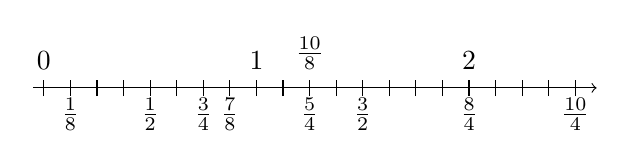
\begin{tikzpicture}[xscale=.27]

	\draw[->]  (-.5,0) -- (26,0);
	\draw  (0,-3pt) -- (0,3pt);
	\draw  (1.25,-3pt) -- (1.25,3pt);
	\draw  (2.5,-3pt) -- (2.5,3pt);
	\draw  (3.75,-3pt) -- (3.75,3pt);
	\draw  (5,-3pt) -- (5,3pt);
	\draw  (6.25,-3pt) -- (6.25,3pt);
	\draw  (7.5,-3pt) -- (7.5,3pt);
	\draw  (8.75,-3pt) -- (8.75,3pt);
	\draw  (10,-3pt) -- (10,3pt);
	\draw  (11.25,-3pt) -- (11.25,3pt);
	\draw  (12.5,-3pt) -- (12.5,3pt);
	\draw  (13.75,-3pt) -- (13.75,3pt);
	\draw  (15,-3pt) -- (15,3pt);
	\draw  (16.25,-3pt) -- (16.25,3pt);
	\draw  (17.5,-3pt) -- (17.5,3pt);
	\draw  (18.75,-3pt) -- (18.75,3pt);
	\draw  (20,-3pt) -- (20,3pt);
	\draw  (21.25,-3pt) -- (21.25,3pt);
	\draw  (22.5,-3pt) -- (22.5,3pt);
	\draw  (23.75,-3pt) -- (23.75,3pt);
	\draw  (25,-3pt) -- (25,3pt);

	\node[above] at (0,3pt)  {0};

	\node[below] at (5,0) {$\frac{1}{2}$};

	\node[above] at (10,3pt)  {1};

	\node[below] at (15,0) {$\frac{3}{2}$};

	\node[below] at (7.5,0) {$\frac{3}{4}$};

	\node[below] at (12.5,0) {$\frac{5}{4}$};

	\node[below] at (20,0) {$\frac{8}{4}$};

	\node[above] at (20,3pt) {2};

	\node[below] at (25,0) {$\frac{10}{4}$};

	\node[below] at (1.25,0) {$\frac{1}{8}$};

	\node[below] at (8.75,0) {$\frac{7}{8}$};

	\node[above] at (12.5,3pt) {$\frac{10}{8}$};
\end{tikzpicture}
\end{center}

\end{atividade}

\begin{atividade}\label{chap3-ativ13}
\objetivos
  \begin{itemize}
   \item Representar frações unitárias na reta numérica.
   \item Comparar frações unitárias na reta numérica.
  \end{itemize}

\discussoes
   \begin{itemize}
   \item  Observe e discuta com seus alunos que, no caso das frações de numerador igual a $1$ (frações unitárias), quanto maior o denominador, menor a fração. Portanto, sua representação na reta numérica está mais perto do zero.
   \item  Aproveite para propor e discutir com seus alunos algumas reflexões tais como:
   \begin{enumerate}[label=\roman*)]
    \item Alguma fração com numerador igual a 1 pode ter sua representação na reta numérica entre $\frac{1}{2}$ e 1?
    \item Qual fração é maior, $\frac{1}{4}$ ou $\frac{1}{10}$?
    \item Que fração tem sua representação na reta numérica mais próxima de 0, $\frac{1}{5}$ ou $\frac{1}{6}$?
   \end{enumerate}

  \end{itemize}

\solucao
As respostas são na ordem I, A, B, H, F, C, E, D e G.

\end{atividade}

\clearpage

\begin{atividade}\label{chap3-ativ14}
\objetivos
  \begin{itemize}
  \item Comparar frações unitárias em sua representação simbólica.
    \end{itemize}

\discussoes
\begin{itemize}
 \item  Nesta atividade, as frações unitárias são apresentadas apenas em sua  representação simbólica. Espera-se que os alunos realizem as comparações mentalmente. Para tal, eles podem se amparar na representação na reta numérica (a exemplo da \hyperref[chap3-ativ13]{atividade anterior}) ou considerar a relação entre os denominadores, ou seja, reconhecendo que a menor é a que tem maior denominador (como já trabalhado na \hyperref[chap2]{Lição 2}).
\end{itemize}

\solucao
\begin{tasks}(2)
\task $\dfrac{1}{2}>\dfrac{1}{5}$.

\task $\dfrac{1}{4}<\dfrac{1}{3}$.

\task $\dfrac{1}{10}>\dfrac{1}{20}$.

\task $\dfrac{1}{12}<\dfrac{1}{2}$.

\task $\dfrac{1}{35}>\dfrac{1}{43}$.

\task $\dfrac{1}{99}>\dfrac{1}{100}$.

\task $\dfrac{1}{5}>\dfrac{1}{50}$.

\task $\dfrac{1}{100}<\dfrac{1}{10}$.
\end{tasks}

\end{atividade}

\begin{atividade}\label{chap3-ativ15}
\objetivos
\begin{itemize} %s
    \item       Comparar frações com o mesmo numerador ou com o mesmo denominador e a partir de um referencial.
\end{itemize} %s

\discussoes
\begin{itemize}
    \item       Estimule seus alunos a explicarem suas respostas.
    \item       A associação das frações aos pontos correspondentes na reta numérica exigirá que os alunos façam comparações de diferentes tipos: frações com mesmo numerador, frações com mesmo denominador e comparação a partir de um referencial (mais detalhes no Para o Professor do início da Lição). Valorize e discuta as diversas estratégias apresentadas por eles.
    \item       Por exemplo, uma vez que os pontos correspondentes ao 0, ao 1 e ao $\frac{1}{2}$ já estão destacados, é natural que as primeiras frações a serem associadas a pontos na reta numérica sejam       $\frac{1}{4}$       e       $\frac{3}{4}$. Em seguida, reconhecendo que       $\frac{1}{8}$       corresponde à metade de       $\frac{1}{4}$,  as frações       $\frac{3}{8}$       e       $\frac{5}{8}$       podem ser as próximas.  Na sequência, o aluno pode reconhecer que       $\frac{4}{5}$       e       $\frac{9}{10}$       são menores do que a unidade e que       $\frac{9}{8}$       e       $\frac{11}{10}$       são maiores.  Entre       $\frac{4}{5}$       e       $\frac{9}{10}$,       $\frac{9}{10}$       pode ser identificada como maior por faltar  apenas       $\frac{1}{10}$       para compor a unidade , enquanto que para       $\frac{4}{5}$       falta       $\frac{1}{5}$       da unidade. Por fim, por raciocínio análogo, a fração       $\frac{9}{8}$       pode ser identificada como maior do que       $\frac{11}{10}$: Sabe-se que $\frac{1}{8}$ é maior do que $\frac{1}{10}$ e que $\frac{9}{8}$  é  $\frac{1}{8}$       maior do que a unidade, enquanto que       $\frac{11}{10}$       é        $\frac{1}{10}$       maior. Portanto, $\frac{9}{8}$    é maior do que       $\frac{11}{10}$.
    \item       Se achar necessário, discuta a comparação entre alguns pares das frações apresentadas antes de os alunos resolverem a atividade. Por exemplo, peça-lhes que comparem       $\frac{3}{8}$        e       $\frac{5}{8}$, que são frações com o mesmo denominador. Ou que comparem       $\frac{9}{8}$       e       $\frac{9}{10}$, frações com o mesmo numerador.
    \item       O aluno pode responder simplesmente       ``ligando''       os cartões com as frações aos pontos correspondentes na reta numérica. No entanto, recomenda-se que o professor oriente-os a escreverm as frações abaixo dos pontos correspondentes na reta numérica, a exemplo do 0, do 1, e do       $\frac{1}{2}$.
\end{itemize} %s

\solucao
\begin{center}
\begin{tikzpicture}
\begin{scope}[scale=.15]
	\draw  (-2,0) -- (45,0);
	\draw[->]  (45,0) -- (47,0);


	\node[below]  at (0,0) {0};						%0
	\node[below]  at (20,0) {$\frac{1}{2}$};		%1/2
	\node[below]  at (40,0) {1};					%1

	\node[below]  at (10,0) {$\frac{1}{4}$};			%1/4
	\node[below]  at (15,0) {$\frac{3}{8}$};			%3/8

	\node[below]  at (25,0) {$\frac{5}{8}$};			%5/8
	\node[below]  at (30,0) {$\frac{3}{4}$};			%3/4
	\node[below]  at (32,0) {$\frac{4}{5}$};			%4/5
	\node[below]  at (36,0) {$\frac{9}{10}$};			%9/10

	\node[below]  at (43.5,0) {$\frac{11}{10}$};		%11/10
	\node[below]  at (45.5,0) {$\frac{9}{8}$};			%9/8
\end{scope}

	\foreach \x in {0,10,15,20,25,30,32,36,40,44,45} \fill[common] (\x*.15,0) circle (2pt);

\end{tikzpicture}
\end{center}
\end{atividade}

\clearpage

\begin{atividade}\label{chap3-ativ16}
\objetivos
  \begin{itemize}
  \item Comparar frações.
  \end{itemize}

\discussoes

   \begin{itemize}
  \item Nesta atividade, as frações são apresentadas apenas em sua representação simbólica. Espera-se que os alunos consigam compará-las a partir da ideia de quantidade e de estratégias mentais. No entanto, é importante observar que alguns alunos podem precisar do apoio de representações diversas. Portanto, a discussão de cada item deve ser amparada por, pelo menos, uma das três estratégias destacadas: (i) argumentação verbal; (ii) representação em modelo contínuo de área e (iii) representação na reta numérica. Por exemplo, na correção do item a), entre $\frac{3}{6}$ e $\frac{5}{6}$, espera-se que a discussão contemple:

   \begin{enumerate}[label=\roman*)]
    \item O fato de que, como essas frações indicam quantidades de ``sextos'', a menor (maior) é aquela que têm menor (maior) numerador. Portanto, $\frac{3}{6}< \frac{5}{6}$.
    \item A representação em modelos contínuos de área.
\begin{center}
      \begin{tikzpicture}[x=56.25mm,y=56.25mm, scale=.6]
\filldraw [fill=common, fill opacity=.3] (0,0) rectangle (1,.1);
\draw[fill=attention] (0,0) rectangle (.5,.1);
\foreach \x in {.167,.333,.5,.667, .833} \draw (\x,0) -- (\x,.1);
\begin{scope}[yshift=-20]
\filldraw [fill=common, fill opacity=.3] (0,0) rectangle (1,.1);
\draw[fill=attention] (0,0) rectangle (.833,.1);
\foreach \x in {.167,.333,.5,.667, .833} \draw (\x,0) -- (\x,.1);
\end{scope}
\end{tikzpicture}
\end{center}
   %cap3:secoes:comparacao_sextos.jpg retângulo da atividade 5 indicando 2/5 e 2/7.
    \item A representação na reta numérica. 
      \begin{center}
        \begin{tikzpicture}[x=5cm]
          \draw [->] (-.2,0) -- (1.2,0);
          \foreach \x in {1,...,5}{
            \draw (\x/6,3pt) -- (\x/6,-3pt);
            \node [below] at (\x/6,0) {$\frac{\x}{6}$};
          }
          \foreach \x in {0,1}{
          \draw (\x,3pt) -- (\x,-3pt);
          \node [below] at (\x,0) {$\x$};
          }
            \fill [common] (.5,0) circle (3pt);
            \fill [common] (.833,0) circle (3pt);
            
        \end{tikzpicture}
      \end{center}
    \end{enumerate}
\end{itemize}

\solucao
\begin{tasks}(3)
\task $\dfrac{5}{9} > \dfrac{4}{9}$

\task $\dfrac{3}{6} < \dfrac{5}{6}$

\task $\dfrac{27}{10} < \dfrac{29}{10}$

\task $\dfrac{3}{12} < \dfrac{9}{12}$

\task $\dfrac{139}{100} >\dfrac{125}{100}$

\task $\dfrac{1}{2} > \dfrac{1}{3}$

\task $\dfrac{1}{7} < \dfrac{1}{6}$

\task $\dfrac{2}{5} > \dfrac{2}{7}$

\task $\dfrac{4}{5} < \dfrac{4}{3}$

\task $\dfrac{12}{15} < \dfrac{12}{7}$

\task $\dfrac{22}{80} > \dfrac{22}{90}$

\task $\dfrac{3}{2} > \dfrac{2}{5}$

\task $\dfrac{3}{4} < \dfrac{6}{5}$

\task $\dfrac{7}{8} < \dfrac{10}{9}$

\task $\dfrac{6}{5} > \dfrac{12}{9}$

\task $\dfrac{4}{5}< \dfrac{5}{4}$

\task $\dfrac{35}{40}< \dfrac{30}{25}$

\task $\dfrac{99}{100}<\dfrac{3}{2}$
\end{tasks}

\end{atividade}

\begin{atividade}\label{chap3-ativ17}
\objetivos
\begin{itemize} %s
    \item       Relacionar a representação de frações unitárias em modelo de área retangular com a representação dessas frações na reta numérica.
\end{itemize} %s

\discussoes
\begin{itemize} %s
    \item  Cada aluno deve receber o material para o desenvolvimento da atividade, que consiste em uma folha, disponível para reprodução no final do livro. Será necessário traçar uma reta. Distribua uma folha para isso ou oriente os alunos a fazê-lo no caderno, usando em ambos os casos a maior dimensão do papel.
    \item Recomenda-se que os alunos manuseiem o material a ser reproduzido. É importante que reconheçam que todos os retângulos coloridos são iguais (congruentes), o que pode ser constatado pela sobreposição. O retângulo representa a unidade. Além disso, é importante que percebam que cada um dos retângulos coloridos (ou a unidade) tem uma equipartição indicada, representando frações unitárias diferentes. Por exemplo, cada parte do retângulo vermelho representa       $\frac{1}{5}$       da unidade.
    \item       Algumas das frações indicadas para serem representadas na reta numérica são maiores que uma unidade. Nesses casos, oriente seus alunos a fazer a justaposição das partes dos retângulos correspondentes. Por exemplo, para representar       $\frac{12}{7}$       será necessário justapor um retângulo a cinco partes do retângulo azul.
\end{itemize} %s

\solucao
\begin{enumerate}
\item Da esquerda para a direita as frações são 1, $\frac{1}{2}$, $\frac{1}{3}$, $\frac{1}{4}$, $\frac{1}{5}$, $\frac{1}{6}$, $\frac{1}{7}$, $\frac{1}{8}$, $\frac{1}{9}$, $\frac{1}{10}$ e $\frac{1}{16}$.


\item \adjustbox{valign=t}
{
\begin{tikzpicture}[x=37mm,y=35mm]
\draw[->] (-.1,0) -- (2.1,0);
\foreach \x in {0,1,2} {\draw (\x,-3pt) -- (\x,3 pt); \node at (\x,10pt) {\x};}
%\node at (60,-20pt) {1};
\foreach \x in {2,3,4} {\fill[common] (1/\x,0) circle (2 pt);\node at (1/\x,-10pt) {$\frac{1}{\x}$};}
\fill[common] (.75,0) circle (2 pt);\node at (.75,-10pt) {$\frac{3}{4}$};
\fill[common] (.6,0) circle (2 pt);\node at (.6,-10pt) {$\frac{3}{5}$};
\fill[common] (5/6,0) circle (2 pt);\node at (5/6,-10pt) {$\frac{5}{6}$};
\fill[common] (7/6,0) circle (2 pt);\node at (7/6,-10pt) {$\frac{7}{6}$};
\fill[common] (6/7,0) circle (2 pt);\node at (6/7,10pt) {$\frac{6}{7}$};
\fill[common] (10/7,0) circle (2 pt);\node at (10/7,10pt) {$\frac{10}{7}$};
\fill[common] (12/7,0) circle (2 pt);\node at (12/7,10pt) {$\frac{12}{7}$};
\fill[common] (10/8,0) circle (2 pt);\node at (10/8,-10pt) {$\frac{10}{8}$};
\fill[common] (12/8,0) circle (2 pt);\node at (12/8,-10pt) {$\frac{12}{8}$};
\fill[common] (10/9,0) circle (2 pt);\node at (10/9,10pt) {$\frac{10}{9}$};
\fill[common] (12/9,0) circle (2 pt);\node at (12/9,-10pt) {$\frac{12}{9}$};
\fill[common] (1,0) circle (2 pt);\node at (1,-10pt) {$\frac{10}{10}$};
\fill[common] (20/16,0) circle (2 pt);\node at (20/16,10pt) {$\frac{20}{16}$};
\end{tikzpicture}
}
\end{enumerate}
\end{atividade}

\clearpage

\begin{atividade}\label{chap3-ativ18}
\objetivos
\begin{itemize} %s
    \item       Representar frações na reta numérica.
    \item       Comparar frações a partir de sua representação na reta numérica.
\end{itemize} %s

\discussoes
\begin{itemize}
    \item       A associação das frações aos pontos correspondentes exigirá que os alunos façam comparações de diferentes tipos. Valorize e discuta as diversas estratégias apresentadas pelos alunos.
    \item Observe que apenas os pontos correspondentes ao 0 e ao 2 estão destacados na reta. Fique atento se seu aluno consegue identificar corretamente a unidade (explícita ou implicitamente). Essa identificação tem papel fundamental na reta numérica. Respostas como as que estão a seguir revelam tal dificuldade.
      \begin{center}
      \begin{tikzpicture}[x=12mm,y=15mm]
\draw[->] (-0.5,0) -- (5.5,0) ; %reta anterior
\foreach \x in {.5, 1, 1.5, 2.5}{ \fill[common] (\x,0) circle (2pt);}
\foreach \x in {0,2}
{
  \draw (\x,-3pt) -- (\x,3pt);
  \node [below] at (\x,0) {\x};
}
\foreach \x in {1,3,5} \node[above] at (\x/2,0) {$\frac{\x}{4}$};
\node[below] at (1, 0) {$\frac{1}{2}$};

\begin{scope}[yshift=-40]
  \draw[->] (-0.5,0) -- (5.5,0) ; %reta anterior
\foreach \x in {.2, .4, .6, 1}{ \fill[common] (\x,0) circle (2pt);}
\foreach \x in {0,2}
{
  \draw (\x,-3pt) -- (\x,3pt);
  \node [below] at (\x,0) {\x};
}
\foreach \x in {1,3,5} \node[above] at (\x/5,0) {$\frac{\x}{4}$};
\node[below] at (.4, 0) {$\frac{1}{2}$};
 \draw (.8,-3pt) -- (.8,3pt);
\node[below] at (.8, 0) {1};
\end{scope}
      \end{tikzpicture}
      \end{center}
    \item       O último item desta atividade admite várias respostas. Explore as soluções dadas pelos seus alunos. Aproveite para discutir estratégias variadas de comparação. Por exemplo, decidir que $\frac{7}{2} < \frac{11}{3} < 4$ pode ser justificado da seguinte maneira: como $4 = \frac{8}{2} = \frac{12}{3}$, na reta, os pontos correspondentes aos números $\frac{7}{2}$ e $\frac{11}{3}$ estarão ambos antes do 4 e, como  $\frac{1}{3} < \frac{1}{2}$, a marcação de $\frac{7}{2}$ estará mais distante de 4 do que a de $\frac{11}{3}$, ou seja, $\frac{7}{2}$ é menor do que~$\frac{11}{3}$.
    \end{itemize} %s

\solucao
\begin{center}
\begin{tikzpicture}[x=12mm,y=15mm]
\draw[->] (-0.5,0) -- (5.5,0) ; %reta anterior
\foreach \x in {0,.25, .5, .75,1, 1.25, 2, 3, 3.5, 3.333, 11/3, 15/4, 4, 17/4, 4.5, 14/3, 5}{ \fill[common] (\x,0) circle (2pt);}
\foreach \x in {1,3,5,15,17} \node[above] at (\x/4,4pt) {$\frac{\x}{4}$};
\foreach \x in {10,11,14} \node[below] at (\x/3, -4pt) {$\frac{\x}{3}$};
\foreach \x in {1,7,9} \node[above] at (\x/2, 4pt) {$\frac{\x}{2}$};
\node[below] at (0,0) {0};
\node[below] at (1,0) {1};
\node[below] at (2,0) {2};
\node[below] at (3,0) {3};
\node[below] at (4,0) {4};
\node[below] at (5,0) {5};

\end{tikzpicture}
\end{center}


\begin{enumerate}
    \item      O número 1 é o ponto que está a mesma distância do 0 e do 2, ou seja, o ``ponto médio'' entre o 0 e o 2. O número $\frac{1}{2}$ é o ponto médio entre o 0 e o 1.

\item  As marcações do $\frac{1}{4}$, $\frac{3}{4}$ e $\frac{5}{4}$ podem ser feitas de maneira semelhante (i) $\frac{1}{4}$ é o ponto médio entre $\frac{1}{2}$ e 1, (ii) $\frac{3}{4}$ é o ponto médio entre $\frac{1}{2}$ e 1, (iii) $\frac{5}{4}$ é o ponto médio entre 1 e $\frac{3}{2}$.
    \item       $\frac{1}{4}$       é menor do que       $\frac{1}{2}$       porque $\frac{1}{4}$ está antes na reta numérica.
    \item       $\frac{3}{4}$       é maior do que        $\frac{1}{2}$       porque $\frac{3}{4}$ está mais adiante na reta numérica.
    \item       $\frac{5}{4}$       é menor do que 1 porque $\frac{5}{4}$ está mais adiante na reta numérica.
    \item       $$0 < \frac{1}{4} < \frac{1}{2}< \frac{3}{4} < 1 < \frac{5}{4} < 2.$$
    \item \mbox{ }
      
      \begin{enumerate}
    \item Há várias respostas possíveis. Por exemplo,       $3 < \frac{7}{2} < 4$,       $3 < \frac{15}{4} < 4$         ou         $3 < \frac{10}{3} < 4$.
    \item       Há várias respostas possíveis. Por exemplo,       $\frac{7}{2} < \frac{15}{4} < 4$ ou $\frac{7}{2} < \frac{11}{3} < 4$.
    \item       Há várias respostas possíveis. Por exemplo,       $\frac{17}{4} < \frac{9}{2} < 5$, $\frac{17}{4} < \frac{19}{4} < 5$ ou $\frac{17}{4} < \frac{14}{3} < 5$.
      \end{enumerate}
     
\end{enumerate} %s

\end{atividade}
